\documentclass{article}
\usepackage[utf8]{inputenc}
\usepackage{polyglossia}
\usepackage{amssymb,amsmath,amsthm}
\usepackage{bussproofs}
\usepackage{enumitem}
\usepackage{fontspec}
\usepackage{tabularx}
\setdefaultlanguage{russian}
\setotherlanguage{english}
\usepackage{translator}
\uselanguage{russian}
\languagepath{russian}
\setmainfont[Ligatures={TeX,Historic}]{CMU Serif}
\setsansfont{CMU Sans Serif}                    %% задаёт шрифт без засечек
\setmonofont{CMU Typewriter Text}               %% задаёт моноширинный шрифт
\usepackage[a4paper, margin=0.5cm]{geometry}
\usepackage{listings}
\usepackage{graphicx}
\pagenumbering{gobble}
%opening
\title{}
\author{}

\begin{document}

%\maketitle
%https://www.youtube.com/playlist?list=PLlb7e2G7aSpS634rDf15afbmKJRSYmH50

\section*{Измерения SAT-Solver}


\begin{tabularx}{0.8\textwidth} { 
	| >{\raggedright\arraybackslash}X 
	| >{\raggedright\arraybackslash}X 
	| >{\raggedright\arraybackslash}X 
  | >{\raggedright\arraybackslash}X
  | >{\raggedright\arraybackslash}X
	| >{\raggedright\arraybackslash}X  | }
   \hline
   Laptop & CPU & OS & RAM & .NET version  & Configuration\\
   \hline
   HP Victus 16& Ryzen 5 5600H  & Ubuntu 22.10  & 16 GB & 6.0.116 & Release  \\
  \hline
  \end{tabularx}

\subsubsection*{Подготовка к измерениям}
Производительность солвера измерялась на 3-CNF SAT наборе из 100 переменных и 499 дизъюнкта. 
Перед измерениями была зафиксирована частота процессора на 3.3 GHz, 
а также закрыты IDE, браузер, мессенджеры и т.д. 
Поскольку первое измерение заметно больше остальных по времени, солвер сначала "разгоняется", разрешая формулу 40 раз.

\subsubsection*{Сырые данные}
После 40 запусков солвера были получены следующие результаты времени работы:
1.678, 1.667, 1.662, 1.644, 1.657, 1.665, 1.664, 1.649, 
1.651, 1.651, 1.661, 1.696, 1.669, 1.676, 1.652, 1.66, 
1.66, 1.662, 1.647, 1.652, 1.654, 1.65, 1.667, 1.662, 1.66,
 1.665, 1.67, 1.671, 1.677, 1.662, 1.673, 1.667, 1.673, 1.676,
  1.667, 1.679, 1.672, 1.68, 1.667, 1.668.




\subsubsection*{Гистограмма и p-value}

\[ \text{ Стандартное отклонение среднего: } \sigma_{msd} = \frac{\sigma_{sd}}{\sqrt{n}}  \]
\begin{figure}[h]
  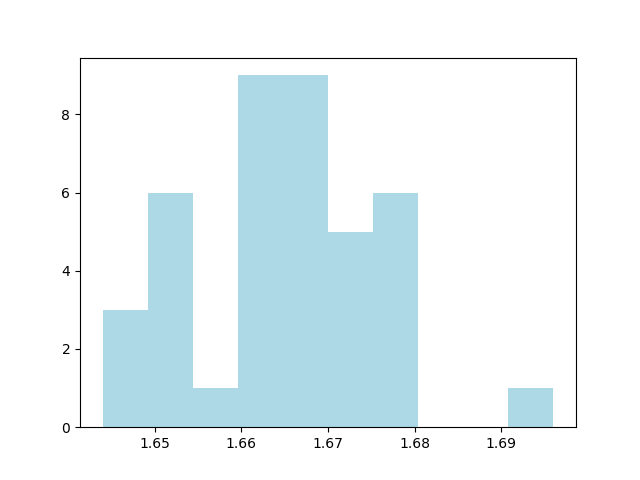
\includegraphics[height=10cm]{Figure_2.png}
\end{figure}

\begin{tabularx}{0.8\textwidth} { 
	| >{\raggedright\arraybackslash}X 
	| >{\raggedright\arraybackslash}X 
	| >{\raggedright\arraybackslash}X 
  | >{\raggedright\arraybackslash}X 
	| >{\raggedright\arraybackslash}X  | }
   \hline
   Среднее значение & Стандартное отклонение  & Стандартное отклонение среднего & p-value normaltest & p-value shapiro \\
   \hline
   1.6646 & 0.0107 & 0.0017  & 0.4241 & 0.4537\\
  \hline
  \end{tabularx}

  \subsubsection*{Доверительный и предсказывающий интервалы}
  \[ \text{ Доверительный интервал: } \overline{x} \pm 2 \cdot \sigma_{msd} \]
  \[ \text { Предсказывающий интервал: } \overline{x} \pm 2 \cdot \sigma_{sd} \]

  \begin{tabularx}{0.8\textwidth} { 
    | >{\raggedright\arraybackslash}X  
    | >{\raggedright\arraybackslash}X  | }
     \hline
     95 Доверительный интервал & Предсказывающий интервал \\
     \hline
       1.66 \pm 0.003 & 1.66 \pm 0.02  \\
    \hline
    \end{tabularx}
\end{document}

